\documentclass[
    20pt,
    margin=1in,
    innermargin=-4.5in,
]{tikzposter}
\geometry{paperwidth=42in,paperheight=30in}
\usepackage[utf8]{inputenc}
\usepackage{amsmath}
\usepackage{amsfonts}
\usepackage{amsthm}
\usepackage{amssymb}
\usepackage{mathrsfs}
\usepackage{graphicx}
\usepackage{adjustbox}
\usepackage{enumitem}
\usepackage[backend=biber,style=numeric]{biblatex}
\usepackage{emory-theme}

\usepackage{mwe}    % for placeholder images

\addbibresource{refs.bib}

% Set theme parameters
\tikzposterlatexaffectionproofoff
\usetheme{EmoryTheme}
\usecolorstyle{EmoryStyle}

\title{AdvancedHMC.jl: a modular implementation of Stan’s no-U-turn sampler in Julia}
\author{Kai Xu\textsuperscript{1}, Hong Ge\textsuperscript{2}, Will Tebbutt\textsuperscript{2} and Mohamed Tarek\textsuperscript{3}}
\institute{
    \textsuperscript{1}University of Edinburgh, United Kingdom \quad \textsuperscript{2}University of Cambridge, United Kingdom \quad \textsuperscript{3}UNSW Canberra, Australia
}
\titlegraphic{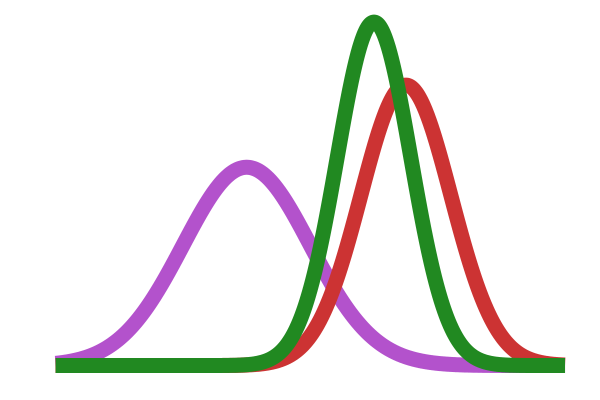
\includegraphics[width=0.075\textwidth]{turing-logo}}

% begin document
\begin{document}
\maketitle
\centering
\begin{columns}

\column{0.32}

\block{Abstract}{
     The No-U-Turn Sampler (NUTS) in Stan has demonstrated remarkable sampling robustness and efficiency in a wide range of Bayesian inference problems, due to the use of self-adaptive Hamiltonian dynamic trajectory simulation length, together with a fine-tuned joint adaptation of step-size and mass matrix. Motivated by these successes, we present AdvancedHMC.jl: a pure Julia implementation of Stan’s built-in NUTS algorithm and related adaptation methods. We hope AdvancedHMC.jl can expose Stan’s NUTS sampling algorithm to a wider range of users, e.g. those who want to write their models by hand, or using a different probabilistic programming language (e.g. Turing, Soss). In our package, a NUTS sampler is defined as a combination of individual components with abstractions including the `Hamiltonian` dynamics, the `Metric` space, how the dynamics are numerically simulated by an Integrator to build up a `Trajectory`, and how a candidate point is sampled from it by a `TrajectorySampler`. This abstraction is partially inspired by “A Conceptual Introduction to Hamiltonian Monte Carlo” by Michael Betancourt.
}

\block{Models}{
    We use five models from MCMCBenchmarks.jl to compare 
    the NUTS implementation between AdvancedHMC.jl and Stan.

    \section{Gaussian Model}

    \section{Signal Detection Model}

    \section{Linear Regression Model}

    \section{Hierarchical Poisson Regression}

    \section{Linear Ballistic Accumulator}
}

\column{0.36}

\block{NUTS Components}{
    AdvancedHMC supports the following combination of different NUTS components.
    $$
    Metric \times Integrator \times TrajectorySampler \times TerminationCriterion \circ Adaptor,
    $$
    where 
    \begin{equation*}
        \begin{aligned} 
            Metric &=  \{UnitEuclidean, DiagEuclidean, DenseEuclidean\} \\ 
            Integrator &=  \{Leapfrog\} \\
            TrajectorySampler &=  \{Slice, Multinomial\} \\
            TerminationCriterion &= \{ClassicNoUTurn, GeneralisedNoUTurn\}
        \end{aligned}
    \end{equation*}
    and $Adaptor$ could be a compositional adaptor with $M$ base adaptors
    $$
    Adaptor = BaseAdaptor_1 \circ BaseAdaptor_2 \cdots \circ BaseAdaptor_M,
    $$
    where 
    $$
    BaseAdaptor \in \{Preconditioner, NesterovDualAveraging\}.
    $$
    Note: $Preconditioner$ will behave differently on different metric spaces.
}

\block{Inference Results}{
    Put plots for inference results and adaptation results.
}

\column{0.32}
\block{Performance}{
    Put plots for performance.
}

\block{Remarks}{
    CuArrays.jl

    Bijectors.jl
}

\block{Acknowledgements}{
    We would like to thank the developers of MCMCBenchmarks.jl, Rob Goedman and Christopher Fisher.
    With this package we run all the benchmarks and generate all the plots used in this poster.
}

\block{References}{
    \vspace{-1em}
    \begin{footnotesize}
    \printbibliography[heading=none]
    \end{footnotesize}
}
    
\end{columns}
\end{document}